\documentclass[11pt]{amsart}

\usepackage[letterpaper,left=125pt,right=125pt]{geometry}

% ^^^^^^^^^^^^^^^^^^^^^^^^^^^^^^^^^^^^^^^^^^^^^^^^^^^^^^^^^^^^^^^^^
\usepackage[english]{babel}
\usepackage {amsmath} 
\usepackage{amssymb}
\usepackage{amsfonts}
\usepackage{amsthm}
\usepackage{graphicx}
\usepackage[dvipsnames]{xcolor}
\usepackage{lipsum}
\usepackage[colorlinks,linkcolor=blue, citecolor=blue,urlcolor=blue]{hyperref}
\usepackage[backend=bibtex]{biblatex}
\usepackage[colorinlistoftodos]{todonotes}
\usepackage{subcaption}

\newcommand{\info}[1]{\todo[linecolor=OliveGreen,backgroundcolor=OliveGreen!25,bordercolor=OliveGreen]{#1}}
\newcommand{\unsure}[1]{\todo[linecolor=red,backgroundcolor=red!25,bordercolor=red]{#1}}
\newcommand{\change}[1]{\todo[linecolor=Plum,backgroundcolor=Plum!25,bordercolor=Plum]{#1}}

%% Environments for theorems, etc.. 
\theoremstyle{theorem} % set the style for the following theorems
\newtheorem{thm}{Theorem}[section] %\newtheorem{name}{display-text}[numbered-within]
\newtheorem{lem}[thm]{Lemma} %\newtheorem{name}[numbered-like]{display-text}
\newtheorem{cor}[thm]{Corollary}
\newtheorem{prop}[thm]{Proposition}
\newtheorem{alg}[thm]{Algorithm}
\theoremstyle{definition}       
\newtheorem{defn}[thm]{Definition}
\newtheorem{conj}[thm]{Conjecture}
\theoremstyle{example}                     
\newtheorem{prob}[thm]{Problem}
\theoremstyle{remark}                       
\newtheorem{exmp}[thm]{Example}
\newtheorem{rem}[thm]{Remark}
\newtheorem{claim}[thm]{Claim}  
\renewcommand{\theclaim}{}

\numberwithin{equation}{section}

\newcommand{\R}{\mathbb{R}}
\newcommand{\Q}{\mathbb{Q}}
\newcommand{\N}{\mathbb{N}}
\newcommand{\Z}{\mathbb{Z}}
\DeclareMathOperator{\rank}{rank}
\DeclareMathOperator{\dimension}{dim}
\DeclareMathOperator*{\supp}{supp}
\DeclareMathOperator{\spn}{span}

\newcommand\numberthis{\addtocounter{equation}{1}\tag{\theequation}}
\usepackage{mwe}

\addbibresource{wavelet.bib}

\title{Haar Wavelet as a Variation on Fourier Series}
\author{Jason Ngo}
\date{2019-05-03}

\begin{document}
\maketitle

\section{Introduction}
Trigonometric polynomials, though most widely used in the computation and study of Fourier series, are not the only orthonormal basis for $ L^2 $. It is known that they exhibit slow convergence and large oscillations near discontinuity points, also known as Gibbs Phenomenon (see Figure \ref{fig:squarewave}). Moreover, the Fourier coefficients, and hence the Fourier series expansion, depend on all values of the function; therefore, if a function $ f $ is changed on a small interval, it is possible that all the Fourier coefficients also change.

\begin{figure}[h]
	\centering
	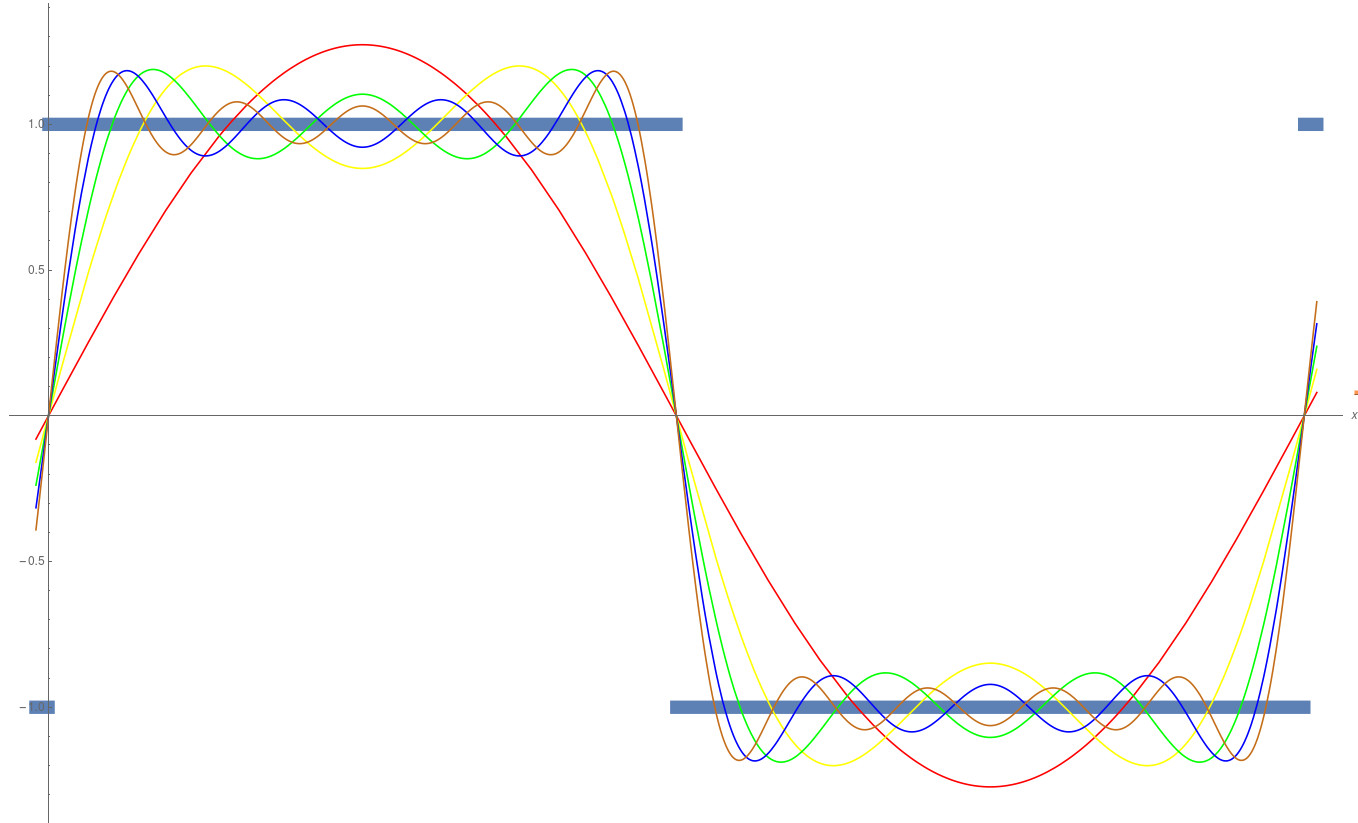
\includegraphics[width=0.4\linewidth]{img/square_wave.png}
	\caption{Fourier Series and Square Wave \cite{weisstein}}
	\label{fig:squarewave}
\end{figure}

These failings of Fourier series motivate us to look for another expansion with the good properties of trigonometric polynomials (such as orthogonality and translation-invariant) but with better local properties: small change on one interval affects only a few of the series coefficients. This local property that we are seeking is extremely important for the analysis of signals with sudden transitions.

Luckily, bases that have such properties do exist, one of which is the Haar wavelet, first proposed in 1909 by Alfréd Haar and further developed in the 1980s (see Figure \ref{fig:haarsystem} for elements in the Haar system). Since then, we have seen rapid development in the theory of wavelets and its practical importance in various fields, namely signal denoising and image processing.

\begin{figure}[h]
	\centering
	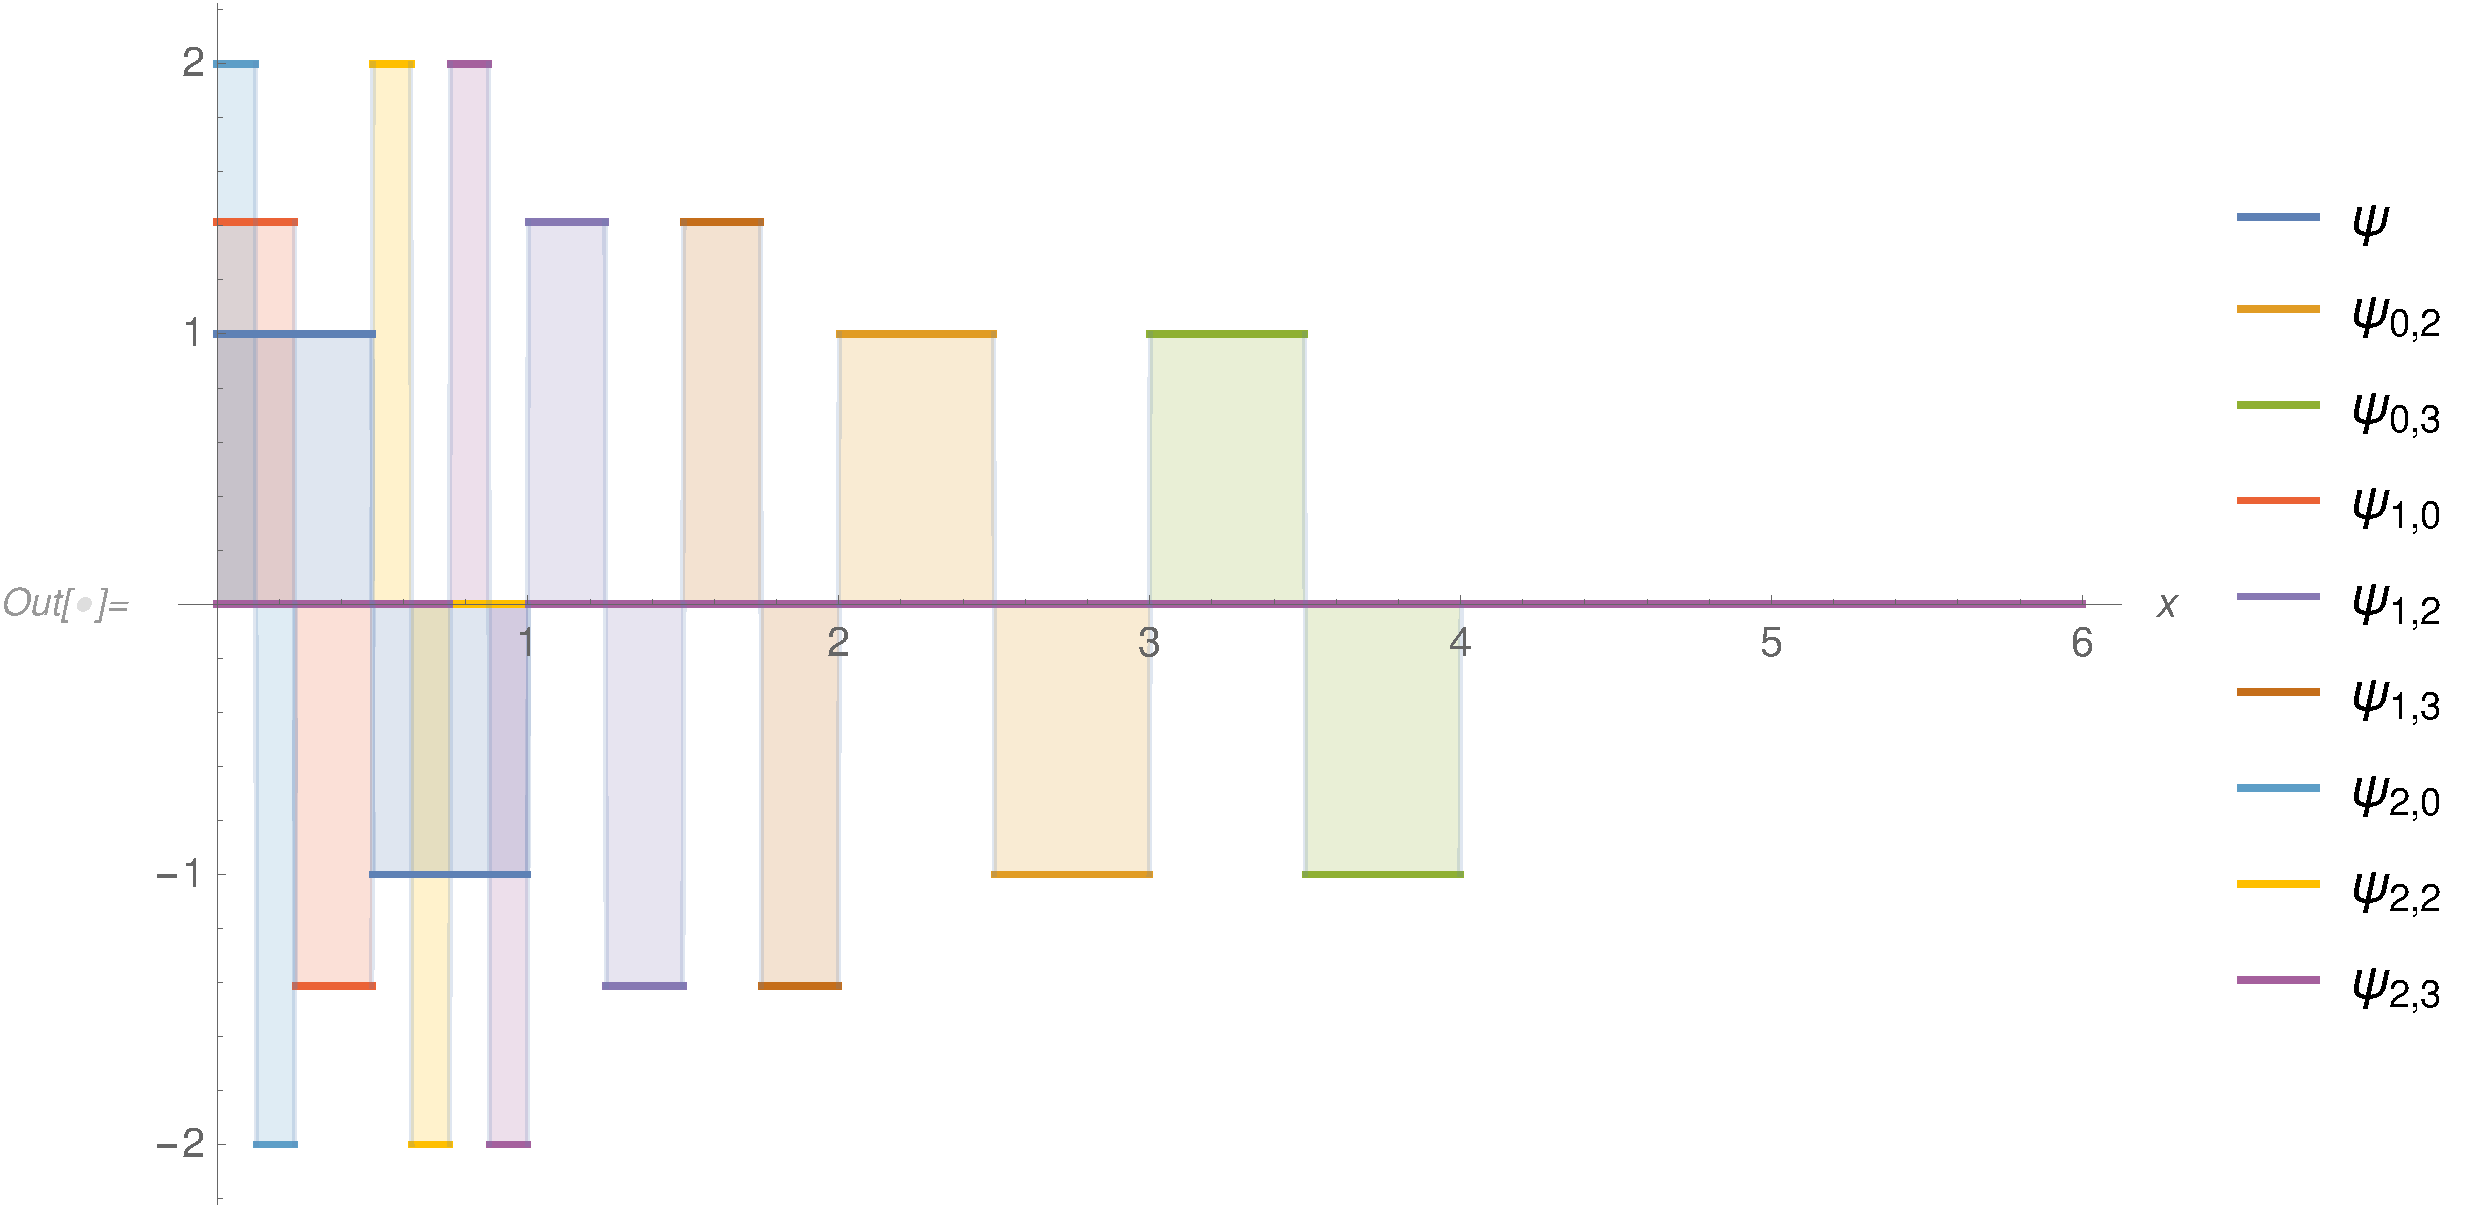
\includegraphics[width=0.7\linewidth]{img/haar_system2}
	\caption[Elements of the Haar system]{Elements of the Haar system}
	\label{fig:haarsystem}
\end{figure}

In this paper, we will prove that the Haar system is an orthonormal basis for $ L^2 $ and discuss its local property advantage over Fourier series expansion.

First, Section \ref{section:def} will provide definitions of the Haar function and of an orthonormal wavelet. In Section \ref{section:orthonormality}, we will prove that the Haar system is orthonormal. Then, Section \ref{section:span} will show that it spans $ L^2(\R) $. Finally, Section \ref{section:application} presents a discussion of the Haar wavelet's local property and the absence of Gibbs phenomenon.

\section{Definition} \label{section:def}
To get started, recall that \emph{$ L^2(\R) $} is a vector space of square integrable functions, taken with the inner product
\[ \langle f,g \rangle = \int_{\R} f(x) g(x)  dx. \]

\begin{defn}[{\cite[515]{davidson}}] \label{haar}
	The \emph{Haar function} is the function $ \varPsi = \chi_{[0,0.5)} - \chi_{[0.5,1)} $. The \emph{Haar system} is the family
	\[ \{ \varPsi_{j,k}(x) = 2^{j/2} \varPsi (2^j x-k) \ | \ j,k \in \Z \}. \]
\end{defn}

	Note that each term in the Haar system is constructed by translating and/or dilating the original $ \varPsi $ (again, see Figure \ref{fig:haarsystem}). By this construction, since $ \int_{\R} \varPsi(x)dx = 0 $, it follows that $ \int_{\R} \varPsi_{j,k}(x)dx = 0 $ for $ j,k \in \Z $.
	Furthermore, it is important to calculate the width and height for each $ \varPsi_{j,k} $. We have $ \varPsi(2^j - k) = 1 $ when $ 0 \leq 2^j - k < \frac{1}{2} $, or equivalently, $ \frac{k}{2^j} \leq x < \frac{k+\frac{1}{2}}{2^j} $. Therefore, in this interval, $ \varPsi_{j,k} = 2^j $. Similar calculations yield:
	\begin{equation} \label{eq:height}
		\varPsi_{j,k} = 
		\begin{cases}
		2^{j/2} &\text{if}\ \frac{k}{2^j} \leq x < \frac{k+\frac{1}{2}}{2^j}, \\
		-2^{j/2} &\text{if}\ \frac{k+\frac{1}{2}}{2^j} \leq x < \frac{k+1}{2^j}, \\
		0 &\text{otherwise}.
		\end{cases}
	\end{equation}
	
Now, we will prove that the Haar function $ \varPsi $ satisfies Definition \ref{def:wavelet} of an \emph{orthonormal wavelet}.

\begin{defn}[Orthonormal Wavelet, {\cite[303]{pinsky}}] \label{def:wavelet}
	If $ \varPsi \in L^2(\R) $, $ \varPsi_{j,k}(x) = 2^{j/2} \varPsi (2^j x-k) $, and the set $ \{ \varPsi_{j,k}: j,k \in \Z \} $ is an orthonormal basis for $ L^2(\R) $, then $ \varPsi $ is called an \emph{orthonormal wavelet}.
\end{defn}

To prove the Haar system is an \textit{orthonormal basis}, we have to show:
	\begin{enumerate}
		\item The Haar system $ \{ \varPsi_{j,k} \} $ is an orthonormal set, i.e. $ \| \varPsi_{j,k} \| = 1 $ for all $ j,k \in \Z $ and $ \langle \varPsi_{j,k}, \varPsi_{j',k'} \rangle = 0 $ for all $ (j,k) \neq (j',k') $.
		
		\item The span of Haar system, denoted $ \spn\{\varPsi_{j,k}\} $, is dense in $ L^2(\R) $.
	\end{enumerate}

\section{Orthonormality} \label{section:orthonormality}
Building upon the terse proof in  \cite{davidson}, this section shows that the Haar system is orthonormal.

\begin{lem}[{\cite[409]{davidson}}] \label{lem:orthonormal}
	The Haar system is an orthonormal set in $ L^2(\R) $.
	
	\begin{proof}
		First, it is easy to see that $ \| \varPsi \| = 1 $. Let us compute:
		\begin{align*}
		\| \varPsi_{j,k} \|^2 = \int_{\R} \left| 2^{j/2} \varPsi(2^{j} x - k) \right|^2 dx 
		&=   \int_{\R} 2^j \left| \varPsi(2^{j} x - k) \right|^2 dx \\
		&= \int_{\R} \left| \varPsi(y) \right|^2 dy
		= \| \varPsi \|^2,
		\end{align*}
		by change of variable $ y = 2^{j}x-k $ in the integral. Therefore, all the elements in the Haar system has norm 1.
		
		Now, we want to show the orthogonality. Consider $ \varPsi_{j,k} $ and $ \varPsi_{j,k'} $, for $ k \neq k' $. Since these two elements have disjoint support\footnote{The \emph{support} of a function, denoted $ \supp $, is the subset of the domain containing those elements which are not mapped to zero.}, their inner product is 0. If $ j < j' $, then either $ \varPsi_{j,k} $ and $ \varPsi_{j',k'} $ have disjoint supports (when $ k \neq k' $), or supp $ \varPsi_{j',k'} $ is contained in an interval on which $ \varPsi_{j,k} $ is constant to $ 2^{j/2} $ (when $ k = k' $). For the former case, their inner product is obviously 0; for the latter case, we have:
		\[ \langle \varPsi_{j,k}, \varPsi_{j',k'} \rangle =  \int_{\R} 2^{j/2} \cdot \varPsi_{j',k'} dx = 2^{j/2} \int_{\R} \varPsi_{j',k'} dx = 0. \]
	
		Hence, the set is orthonormal.
	\end{proof}
\end{lem}

\begin{rem}
	The Haar function is a dyadic function, meaning that the dilations are taken to be powers of 2. Here, the factor $ 2^{j/2} $ is called the normalization factor, which is there so that the dilated and translated Haar function has norm 1. Although powers of 2 are a common choice, they are certainly not the most general one\footnote{See examples of non-dyadic wavelets and a discussion why they are more appropriate for statistical data analysis in \cite{pollock}.}.
\end{rem}

\section{Haar Wavelet Basis for $ L^2(\R) $} \label{section:span}
Now that we have shown the Haar system is orthonormal, this section will finish showing $ \varPsi $ satisfies Definition \ref{def:wavelet} by proving the following theorem:

\begin{thm}[{\cite[411]{davidson}}] \label{thm:span}
	The Haar system $ \{ \varPsi_{j,k} \} $ spans all of $ L^2(\R) $.
\end{thm}

To prove this theorem, we will start out with $ C_c(\R) $, the set of continuous functions with compact support. Since $ C_c(\R) $ is dense in $ L^2(\R) $\footnote{The proof that $ C_c(\R) $ is dense in $ L^2(\R) $ can be found in \cite[326]{farrell}.}, if we can show that any function $ f \in C_c(\R) $ is in the closure of the span of $ \{\varPsi_{j,k}\} $, then it follows that $ \{ \varPsi_{j,k} \} $ spans $ L^2(\R) $.

Motivated by \cite[3]{bell} and \cite[516]{davidson}, we will set up the integral transform $ P_nf $ in Section \ref{subsec:integral transform}, and then in Section \ref{subsec:two-sided}, we proceed to define the Haar inner product expansion and prove that it is dense in $ C_c(\R) $. 

\subsection{Integral Transform} \label{subsec:integral transform}
Set $ \phi(x) = \chi_{[0,1)}$. For $ n \in \Z $, we define the integral kernel
\[ K_n (x,y) = 2^n \sum_{k \in \Z} \phi(2^n x - k) \phi(2^n y - k). \]

Note that $ K_n $ is either equal to $ 2^n $ (when there is some $ k \in \Z $ s.t. $ 2^n x-k $ and $ 2^ny - k $ lie in $ [0,1) $) or equal to 0 (otherwise). In other words, if $ K_n = 2^n $, then there is some $ k $ s.t.
\begin{equation} \label{eq:K}
	x,y \in \left[ \frac{k}{2^n}, \frac{k+1}{2^n} \right) = I_{n,k}.
\end{equation}
Here, note that each $ I_{n,k} $ has length $ 2^{-n} $ and that
the sets $ \{ I_{n,k} \} $ are disjoint.

We define the integral transform
\[ P_n f(x) = \int_{\R} K_n(x,y) f(y) dy. \]
If $ x \in \R $ then there is a unique $ k_x \in \Z $ with $ x \in I_{n, k_x} $ and
\begin{equation} \label{eq:pnf}
	P_n f(x) = 2^n \int_{I_{n,k_x}} f(y) dy.
\end{equation}
Since $ I_{n,k_x} $ has length $ 2^{-n} $, we can say that $ P_nf $ is the average value of a function $ f $ on the dyadic interval containing $ x $.

\vspace{8pt}
Notice that the integral kernel $ K_n $ is dependent on $ \phi $. In order to write any function in terms of the Haar system $ \{ \varPsi_{j,k} \} $, we must eliminate $ \phi $ somehow from our calculations. The following Lemma \ref{lem:expansion} will write the integral kernels in terms of $ \{ \varPsi_{j,k} \} $.

\begin{lem}[{\cite[293]{pinsky}}] \label{lem:expansion}
	If $ n \in \Z $, then
	\[ K_{n+1} - K_n = \sum_{k \in \Z} \varPsi_{n,k}(x) \varPsi_{n,k}(y),\qquad x,y \in \R. \]
	
	\begin{proof}
		First, let us calculate the right-hand side.
		By Equation (\ref{eq:height}), $ \varPsi_{n,k}(x) = 2^{n/2} $ when $ x \in I_{n+1,2k} = \left[\frac{2k}{2^{n+1}}, \frac{2k+1}{2^{n+1}}\right) $, and similarly, $\varPsi_{n,k}(x)= -2^{n/2} $ when $ x \in I_{n+1,2k+1}$. Therefore, it follows that:
		\[
		\varPsi_{n,k}(x) \varPsi_{n,k} (y) =
		\begin{cases}
		2^n &\text{if}\ x,y \in I_{n+1,2k}\ \text{or}\ x,y \in I_{n+1,2k+1}, \\
		-2^n &\text{if one is in }\ I_{n+1,2k}\ \text{and the other is in}\ I_{n+1,2k+1}, \\
		0 &\text{otherwise}.
		\end{cases}
		\]
		
		Now, before calculating the left-hand side $ K_{n+1} - K_n $, note that:
		\[
		I_{n+1,2k} \cup I_{n+1,2k+1} = \left[ \frac{2k}{2^{n+1}}, \frac{2k+2}{2^{n+1}} \right) = I_{n,k}. 
		\]
		
		Therefore, if both $ x,y $ are in $ I_{n+1,2k} $ or $ I_{n+1,2k+1} $, then we have (1) $ K_{n+1} = 2^{n+1} $ (by Equation (\ref{eq:K})) and (2) $ K_n = 2^n $ (because $ x,y \in I_{n,k} $), Hence,
		\[ K_{n+1}(x,y) - K_n(x,y) = 2^{n+1} - 2^n = 2^n. \]

		By similar argument, if either $ x $ or $ y $ is in $  I_{n+1,2k} $ and the other is in $ I_{n+1,2k+1} $, then
		$ K_{n+1}(x,y) - K_n(x,y) = 0 - 2^n = -2^n. $ 
		
		Otherwise, both $ K_{n+1} $ and $ K_n $ are 0.
	\end{proof}
\end{lem}

\begin{rem}
	From this Lemma, the difference between two integral transforms can be written as the \textit{inner product expansion} of the function $ f $:
	\begin{align*}
	(P_{n+1} - P_n) f(x) &= \int_{\R} K_{n+1}(x,y)f(y)dy - \int_{\R} K_{n}(x,y)f(y)dy \\
	&= \int_{\R} \sum_{k \in \Z} \varPsi_{n,k}(x) \varPsi_{n,k}(y) f(y) dy \\
	&= \sum_{k \in \Z} \varPsi_{n,k}(x) \int_{\R} \varPsi_{n,k}(y) f(y) dy \\
	&= \sum_{k \in \Z} \langle f, \varPsi_{n,k} \rangle \varPsi_{n,k}(x).  \numberthis \label{eq:expansion}
	\end{align*}
	
	The terms $ \langle f, \varPsi_{j,k} \rangle $ are called the Haar coefficients.
	One can easily notice that this inner product expansion is only one-sided, meaning we keep the dilation factor $ j = n $ fixed and vary the translation factor $ k $. In the next section, we will abstract this expansion to a more general setting, varying both the translation and dilation factors.
\end{rem}


\subsection{Two-sided Haar Representation} \label{subsec:two-sided}
From Equation \ref{eq:expansion}, we can write
\begin{equation} \label{eq:twosided}
	P_{n+1}f(x) - P_{-m}f(x) = \sum_{j=-m}^{n} \sum_{k \in \Z} \langle f, \varPsi_{j,k} \rangle \varPsi_{j,k}(x).
\end{equation}

To prove that any function $ f \in C_c(\R) $ is in the closure of the span of $ \{ \varPsi_{j,k} \} $, we want to show that the Haar inner product expansion on the right-hand side converges to $ f $. By Equation (\ref{eq:twosided}) above, it suffices to show $ P_{-m}f \to 0 $ and $ P_{n+1}f \to f $ with respect to the $ L^2 $ norm as $ m, n \to \infty $. The two claims are presented as Lemmas below.

\vspace{8pt}
First, Lemma \ref{lem:average} tells us that the larger the intervals on which we average a continuous function, the smaller the supremum of the averaged function. The proof below is an extended version of the proof found in \cite{pinsky}, with step-by-step calculations added.

\begin{lem}[Average Function over Dyadic Intervals, {\cite[295]{pinsky}}] \label{lem:average}
	If $ f \in C_c(\R) $, then $ \|P_{-m}f\|_2 \to 0 $ when $ m \to \infty $.
	
	\begin{proof}
		Suppose $ f \in C_c(R) $ and $ \supp(f) \subseteq [-K,K] $. There eixsts $ M > 0 $ s.t. $ \supp(f) \subset [-2^M, 2^M] $. Now, if $ m > M $, then $ \supp(f) \subseteq I_{-m,-1} \cup I_{-m,0} $; Equation (\ref{eq:pnf}) therefore holds.
		We compute:
		\begin{align*}
			\| P_{-m}f \|_2^2 &= \int_{\R} \left| P_{-m}f(x) \right|^2 dx 
			= \sum_{k \in \Z} \int_{I_{-m,k}} |P_{-m}f(x)|^2 dx \\
			&= \sum_{k \in \Z} \int_{I_{-m,k}} \left|2^{-m} \int_{I_{-m,k}} f(y) dy \right|^2 dx
			= 2^{m}  2^{-2m} \sum_{k \in \Z} \left|\int_{I_{-m,k}} f(y) dy \right|^2 dx.
		\end{align*}
		Since $ f $ is only supported on a subset of $ I_{-m,-1} $ and $ I_{-m,0} $, we have:
		\begin{align*}
		\| P_{-m}f \|_2^2	&= 2^{-m} \left( \left|\int_{I_{-m,-1}} f(y) dy \right|^2 dx + \left| \int_{I_{-m,-1}} f(y) dy \right|^2 dx \right) \\
			&=  2^{-m} \left( \left|\int_{-K}^0 g(y) dy \right|^2 dx + \left| \int_{0}^K f(y) dy \right|^2 dx \right).
		\end{align*}
		Note that $ \int_{-K}^0 f(y) dy = \langle f(y),\chi_{[-K,0)}  \rangle $; by Cauchy-Schwarz inequality,
		\begin{align*}
		\| P_{-m}f \|_2^2	&\leq  2^{-m} \left( K \|f\|_2^2 + K \|f\|_2^2 \right) = 2^{-m} \cdot 2K \|f\|_2^2.
		\end{align*}
		As $ m \to \infty $, the right-hand side converges to 0. Therefore, by Squeeze Theorem, it follows that $ \|P_{-m}f\|_2 \to 0 $.
	\end{proof}
\end{lem}

Now, before proving our next Lemma, recall that $ P_nf(x) $ is equal to the average value of a function $ f $ on a small dyadic interval of length $ 2^{-n} $. Therefore, if we increase $ n $, then the intervals will get smaller, and the average value $ P_nf $ will get closer to $ f $ (see Figure \ref{fig:converge} for the sequence $ \{P_nf\} $ approaching $ f(x) = 0.5 + e^{-x} \sin{2\pi x} $ on the unit interval). 

\begin{figure}[h]
	\centering
	\begin{subfigure}[b]{0.475\textwidth}
		\centering
		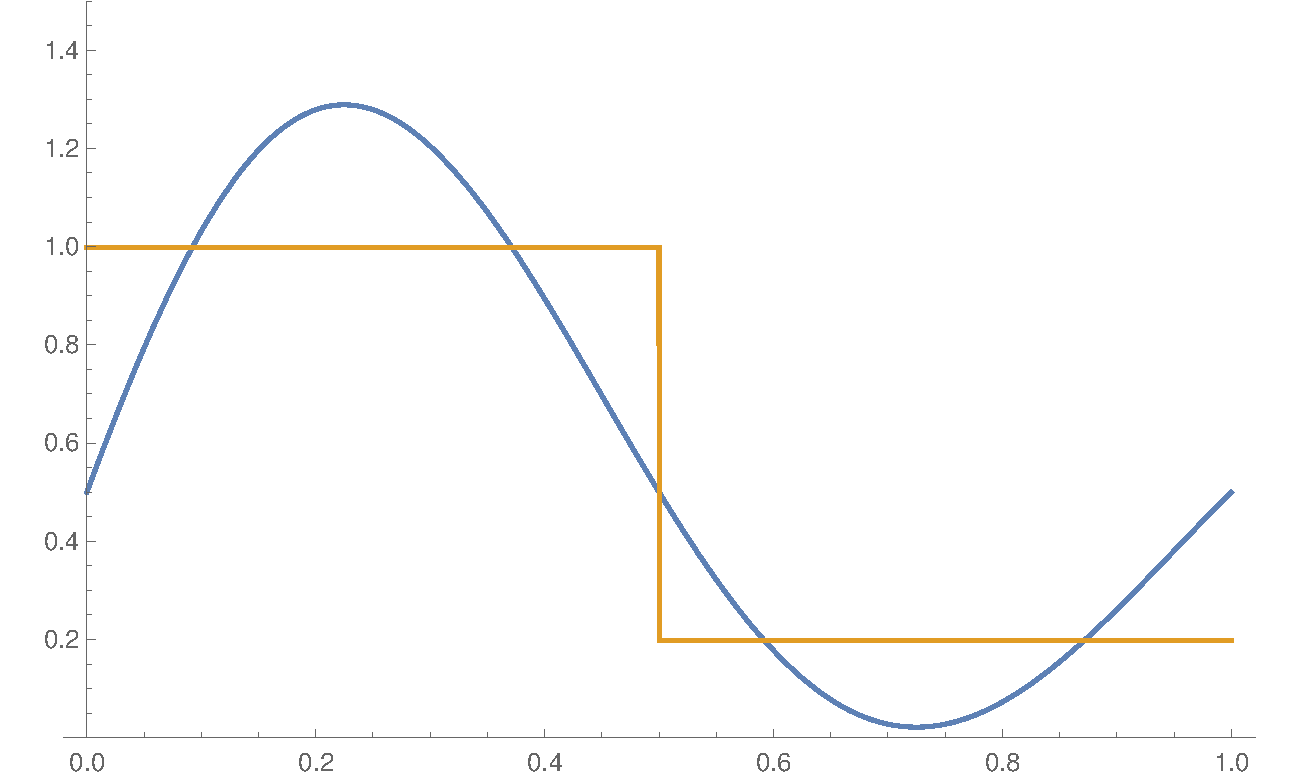
\includegraphics[width=\textwidth,height=0.35\linewidth]{img/e1}
		\caption[Network2]%
		{{\small $ n = 1 $}}    
	\end{subfigure}
	\hfill
	\begin{subfigure}[b]{0.475\textwidth}  
		\centering 
		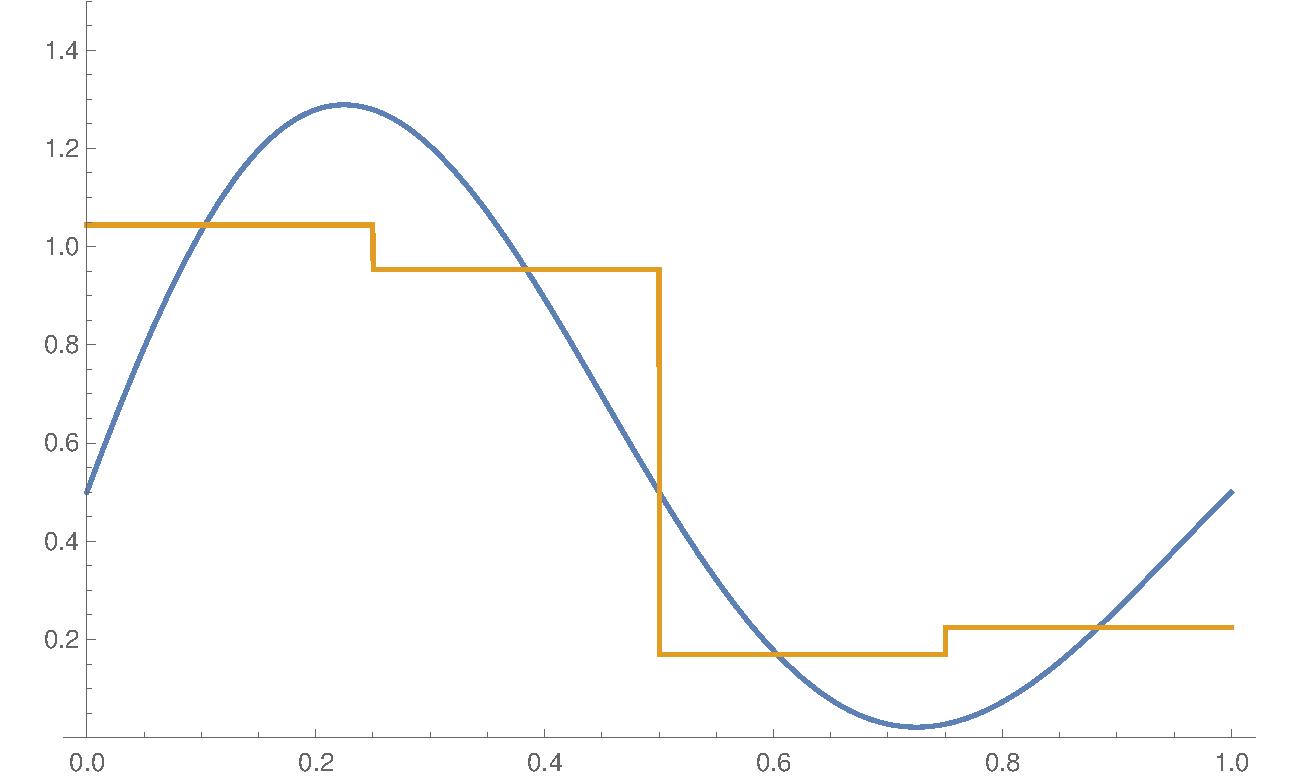
\includegraphics[width=\textwidth,,height=0.35\linewidth]{img/e2}
		\caption[]%
		{{\small $ n = 2 $}}
	\end{subfigure}
	\vskip\baselineskip
	\begin{subfigure}[b]{0.475\textwidth}   
		\centering 
		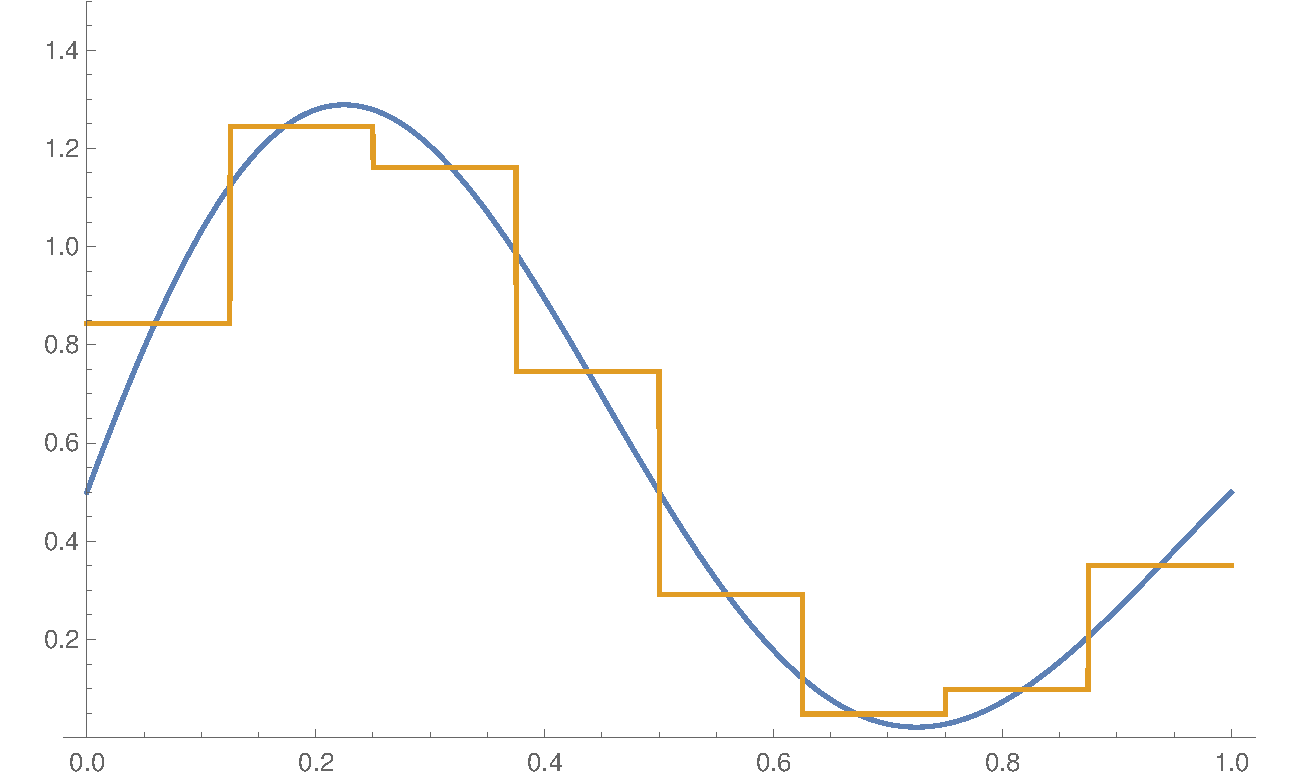
\includegraphics[width=\textwidth,,height=0.35\linewidth]{img/e3}
		\caption[]%
		{{\small $ n = 3 $}}    
	\end{subfigure}
	\quad
	\begin{subfigure}[b]{0.475\textwidth}   
		\centering 
		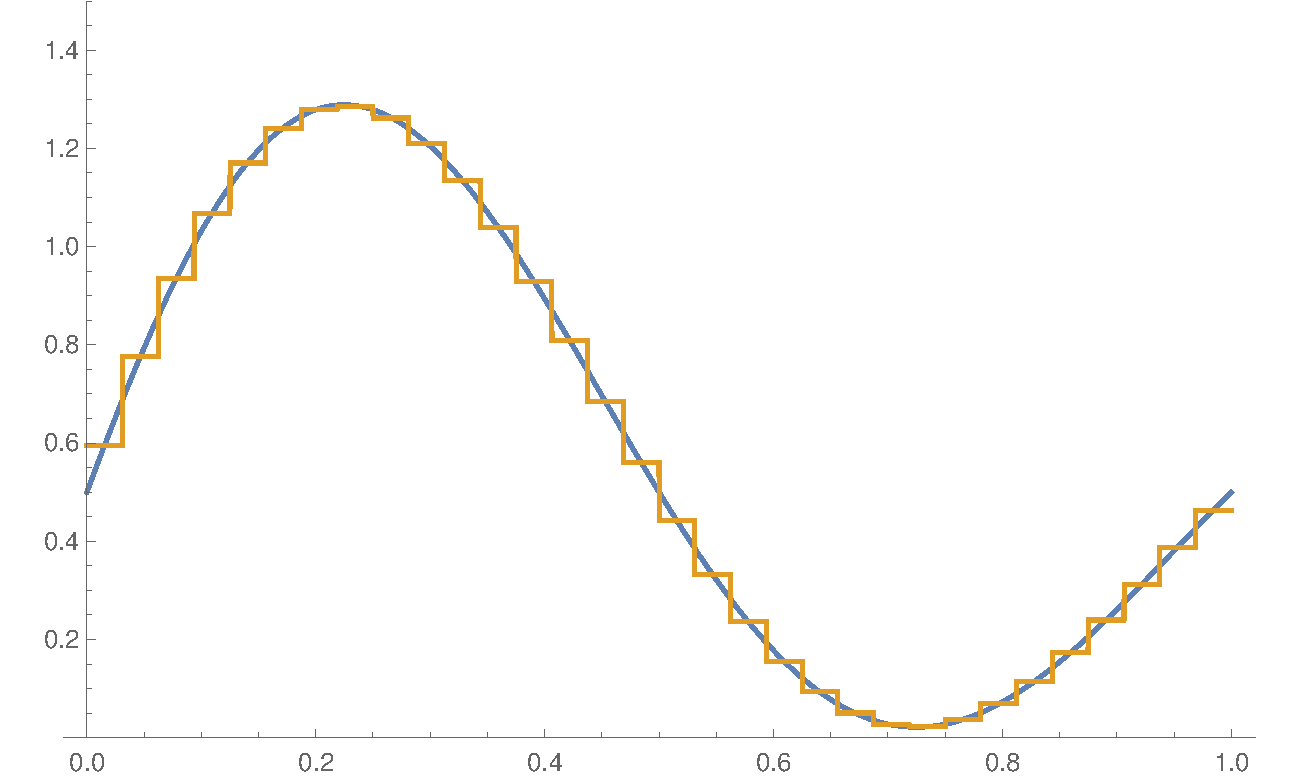
\includegraphics[width=\textwidth,height=0.35\linewidth]{img/e5}
		\caption[]%
		{{\small $ n = 5 $}}    
	\end{subfigure}
	\caption[]
	{Approximation of $ f(x) = 0.5 + e^{-x} \sin{2\pi x} $ by $ P_nf(x) $}
	\label{fig:converge}
\end{figure}

\begin{lem}[Convergence of Integral Transform, {\cite[517]{davidson}}] \label{lem:convergence}
	If $ f \in C_c(\R) $, then $ P_nf \to f $ in the uniform norm as well as in the $ L^2 $ norm.
	
	\begin{proof}
		Suppose $ f \in C_c(\R) $ and $ \supp(f) \subset [-2^M, 2^M] $ for $ M \geq 0 $. Since $ f $ is continuous on a compact set, it is uniformly continuous.
		
		Given $ \epsilon > 0 $. By uniform continuity, there exists $ \delta > 0 $ such that if $ |x-y| < \delta $, then $ |f(x) - f(y)| < \epsilon $.
		
		Now, choose $ N $ such that $ 2^{-N} < \delta $; if $ n > N $, then we have:
		\begin{align*}
		|P_nf(x) - f(x)| &= \left| 2^n \int_{I_{n,k_x}} f(y)dy - f(x) \right| \\
		&=  \left| 2^n \int_{I_{n,k_x}} f(y)dy - 2^n \int_{I_{n,k_x}} f(x) dy \right| \\
		&\leq 2^n \int_{I_{n,k_x}} |f(y) - f(x)| dy 
		< 2^n \int_{I_{n,k_x}} \epsilon dy = \epsilon.
		\end{align*}
		Therefore, $ P_nf $ converges to $ f $ uniformly. Since uniform convergence implies $ L^2 $ convergence, it follows that $ P_nf \to f $ with respect to the $ L^2 $ norm.
	\end{proof}
\end{lem}

Now, we are ready to prove that the Haar system spans all of $ L^2(\R) $:

\begin{proof}[Proof of Theorem \ref{thm:span}]
	By Lemma \ref{lem:average} and Lemma \ref{lem:convergence}, it follows that for any $ f \in C_c(\R) $, 
	\[
	f = \sum_{j \in \Z} \sum_{k \in \Z} \langle f, \varPsi_{j,k} \rangle \varPsi_{j,k}.
	\]
	Since $ C_c(\R) $ is a dense subspace of $ L^2(\R) $, we conclude that the Haar system spans $ L^2(\R) $. The Haar function $ \varPsi $ is therefore an orthonormal wavelet; we will now refer to it as the \emph{Haar wavelet}.
\end{proof}


\section{Haar Wavelet's Local Property} \label{section:application}
In previous sections, we have seen the Haar wavelet has the good properties of trig functions: $ \{ \varPsi_{j,k} \} $ is orthonormal and spans $ L^2(\R) $. Now, in this final section, we will discuss in detail how this Haar wavelet basis helps resolve the issues for which Fourier series work badly.

\subsection{Preservation of Series Coefficients} As opposed to the Fourier coefficients, each Haar coefficient $ \langle f,\varPsi_{j,k} \rangle $ depends only on the values of the function on $ \supp \varPsi_{j,k} $. Therefore, when we change a function on an interval $ E $, only the Haar coefficients with $ \supp \varPsi_{j,k} $ that overlaps with $ E $ change; the rest of the Haar coefficients remain unchanged. The same, unfortunately, cannot be said about Fourier series expansion.

\begin{exmp}
	Consider $ f(x) = 0.5 + e^{-x} \sin{2\pi x} $ and $ g(x) = f(x) + 0.1 \chi_{[0.6,0.61)} $.
\end{exmp}

Using \verb|Mathematica|, we calculate the first 100 Fourier coefficients $ A_n $ of $ f(x) $ and $ g(x) $ and notice that all coefficients change (see Figure \ref{fig:fouriercoeff}). Although these changes are small, they pose a challenge to the computation of Fourier series approximations when we want to modify the pitch of a signal at a given time.

\begin{figure}[h]
	\centering
	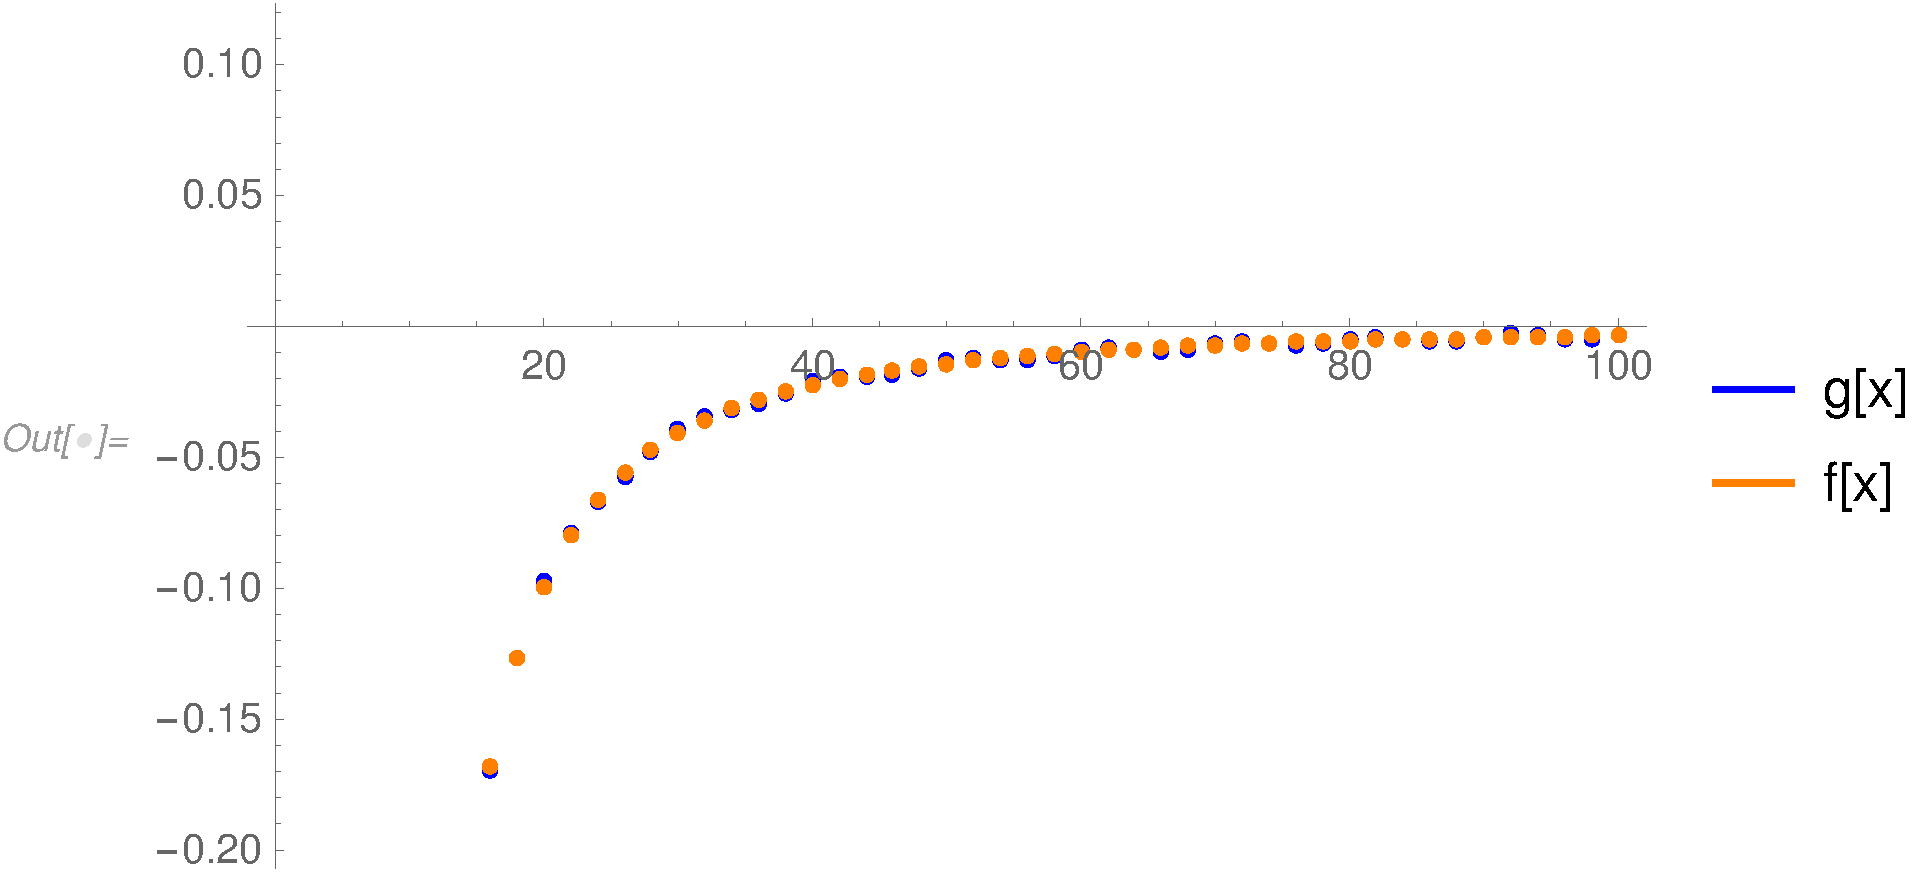
\includegraphics[width=0.5\linewidth]{img/fourier_coeff}
	\caption{Fourier coefficients $ A_n $ of $ f(x) $ and $ g(x) $}
	\label{fig:fouriercoeff}
\end{figure}

\subsection{Gibbs Phenomenon}
Since the square wave presented in Figure \ref{fig:squarewave} is a piecewise constant function, we can be certain that there is no Gibbs phenomenon when we approximate using the Haar wavelet basis, for we can always translate or dilate Haar functions to obtain the square wave. For a more general case, it turns out that the Haar series expansions does not exhibit Gibbs phenomenon when approximating any $ f \in L^2(\R) $ either. The proof for this claim falls outside the scope of this paper; however, it can be found in \cite[Chap. 5]{raeen} and \cite{kelly}.

\printbibliography

\end{document}

